\subsubsection{Uruchomienie kamery}
Do dzia�ania algorytmu SVO jest potrzebny obraz z kamery, kt�ra zosta�a uruchomiona dzi�ki sterownikom zaimplementowanym w paczce \textit{usb\_cam}. Po uruchomieniu algorytmu, nale�y uruchomi� plik launchowy, dostarczaj�cy obraz z kamery. Poni�szy wydruk przedstawia uruchomienie kamery.


\begin{lstlisting}[language=XML, frame=single,tabsize=1, caption={Uruchomienie kamery}] 
<launch>
  <node name="usb_cam" pkg="usb_cam" type="usb_cam_node"
  / output="screen" >
    <param name="video_device" value="/dev/video0" />
    <param name="image_width" value="640" />
    <param name="image_height" value="480" />
    <param name="pixel_format" value="mjpeg" />
    <param name="camera_frame_id" value="usb_cam" />
    <param name="io_method" value="mmap"/>
  </node>
</launch>
\end{lstlisting}

\subsubsection{Kalibracja kamery}
Do uruchomienia algorytmu potrzebny jest plik kalibracyjny. Kalibracj� kamery wykonano standardowym narz�dziem zaimplementowanym w ROSie w paczce  \texttt{camera\_calibration}. Wynikiem tej operacji jest plik *.yml. Na potrzeby algorytmu przkonwertowano plik *.yml na format *.yaml.
\begin{figure}[tp]
\centering
	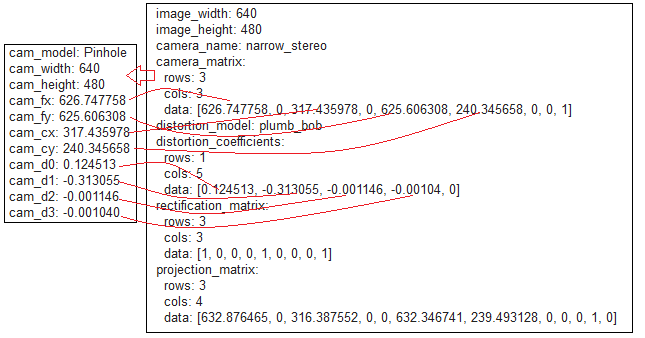
\includegraphics[scale=1]{grafika/kali.png}
	\caption{Konwersja pliku *.yml na *.yaml}
	\label{yml}
\end{figure}
Rysunek \ref{yml} przedstawia r�czne przekonwertowanie pliku kalibracyjnego.
\subsubsection{Pozycja kamery}
Do dalszego przetwarzania informacji dostarczonych z dzia�aj�cej paczki SVO mo�na wykorzysta� wiadomo�� publikowan� poprzez topic \texttt{/svo/points}.
\begin{figure}[tp]
\centering
	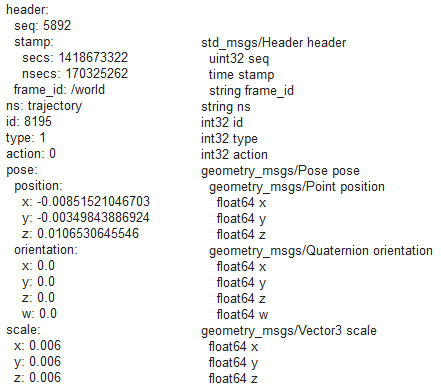
\includegraphics[scale=1]{grafika/topic.png}
	\caption{Wycinek informacji zawartych w topicu \texttt{/svo/points}}
	\label{t}
\end{figure}
Rysunek \ref{t} pokazuje struktur� kluczowego topicu SVO. Typ wiadomo�ci to \textit{visualization\_msgs}. Wiadomo�� ta jest zbiorem informacji u�ywanych przez takie pakiety jak, np. \textit{rviz}. G��wn� wiadomo�ci� w tym topicu jest \textit{visualization\_msgs/Marker}. Do dalszego przetwarzania u�yto komunikatu zawieraj�cego informacj� o pozycji kamery. Mo�na t� informacj� uzyska� poprzez subskrybowanie si� do tego topicu.
\subsubsection{Modyfikacja}
Algorytm SVO posiada w�tek u�ytkownika. Zdecydowano si� na wy��cznie tego w�tku. Program zmodyfikowano tak, by dzia�a� automatycznie, bez czekania na akcj� u�ytkownika, kt�ry decydowa� o starcie algorytmu, przy jego wcze�niejszym resecie.